\documentclass[handout]{beamer}
\usetheme{metropolis}
\beamertemplatetransparentcoveredhigh

\usepackage[portuges]{babel}
\usepackage{graphicx}
\graphicspath{{./figs/}}
\usepackage{listings}
\usepackage{color}
\usepackage{hyperref}
\usepackage{xpatch}
\usepackage{comment}
\usepackage[outputdir=build]{minted}

\makeatletter
\AtBeginEnvironment{minted}{\dontdofcolorbox}
\def\dontdofcolorbox{\renewcommand\fcolorbox[4][]{##4}}
\xpatchcmd{\inputminted}{\minted@fvset}{\minted@fvset\dontdofcolorbox}{}{}
\xpatchcmd{\mintinline}{\minted@fvset}{\minted@fvset\dontdofcolorbox}{}{}
\makeatother
\setminted[c]{
  linenos=true,
  breaklines=true,
  encoding=utf8,
  frame=lines,
  framerule=0.5pt,
  autogobble,
  fontsize=\small,
}
\setminted[bash]{
  linenos=true,
  encoding=utf8,
  frame=lines,
  framerule=0.5pt,
  autogobble,
  fontsize=\small
}

\newcommand{\cod}[1]{\mintinline{c}{#1}}


\definecolor{dkgreen}{rgb}{0,0.6,0}
\definecolor{gray}{rgb}{0.5,0.5,0.5}
\definecolor{mauve}{rgb}{0.58,0,0.82}


\definecolor{Purple}{HTML}{911146}
\definecolor{Orange}{HTML}{CF4A30}
\setbeamercolor{alerted text}{fg=Orange}
\setbeamercolor{frametitle}{bg=Purple}
\setbeamercolor{block body}{bg=Purple!20,fg=black}
\setbeamercolor{block title}{bg=Purple!50,fg=black}
\setbeamertemplate{blocks}[rounded][shadow=true]


\newcounter{ExercicioCounter}
\newcommand{\exercicio}{\refstepcounter{ExercicioCounter} Exercício~\theExercicioCounter}

\newcommand{\setcoverbg}{
  \setbeamertemplate{background}
  {
\includegraphics[width=\paperwidth,height=\paperheight]{backgrounds/coverbg}}
}
\newcommand{\setsectionbg}{
  \setbeamertemplate{background}
  {
\includegraphics[width=\paperwidth,height=\paperheight]{backgrounds/blank}}
}

\title{Programação Estruturada}
\subtitle{Ponteiros --- Parte 2}

\author{Professores Emílio Francesquini e Carla Negri Lintzmayer}
\institute{Centro de Matemática, Computação e Cognição\\ Universidade Federal do ABC}
\date{2018.Q3}

\begin{document}

\setcoverbg
\maketitle
\setsectionbg


%%%%%%%%%%%%%%%%%%%%%%%%%%%%%%%%%%%%%%%%%%
%%%%%%%%%%%%%%%%%%%%%%%%%%%%%%%%%%%%%%%%%%
%%%%%%%%%%%%%%%%%%%%%%%%%%%%%%%%%%%%%%%%%%
%%%%%%%%%%%%%%%%%%%%%%%%%%%%%%%%%%%%%%%%%%
%%%%%%%%%%%%%%%%%%%%%%%%%%%%%%%%%%%%%%%%%%
%%%%%%%%%%%%%%%%%%%%%%%%%%%%%%%%%%%%%%%%%%
\section{Ponteiros}

%%%%%%%%%%%%%%%%%%%%%%%%%%%%%%%%%%%%%%%%%%%%%%
\begin{frame}[fragile]{Ponteiros}

    Lembre-se que uma variável vetor possui um endereço, e que podemos atribuí-la para uma variável ponteiro:
    \vspace{-0.5cm}
    \begin{minted}{c}
        int a[] = {1, 2, 3, 4, 5};
        int *p;
        p = a;
    \end{minted}

    E podemos então usar \cod{p} como se fosse um vetor:
    \vspace{-0.5cm}
    \begin{minted}{c}
        for (i = 0; i < 5; i++)
            p[i] = i*i;
    \end{minted}

    \begin{center}
        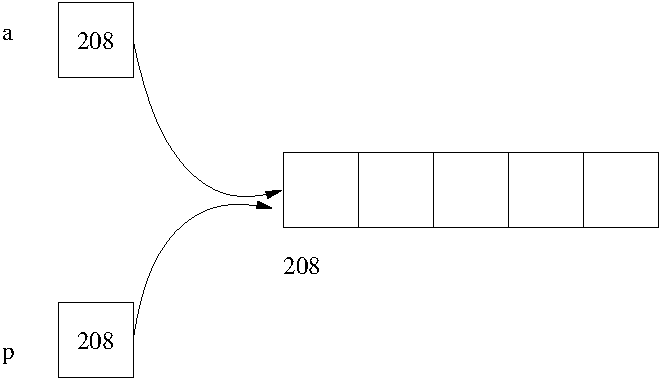
\includegraphics[scale=0.4]{pont}
    \end{center}

\end{frame}

%%%%%%%%%%%%%%%%%%%%%%%%%%%%%%%%%%%%%%%%%%%%%%
\begin{frame}[fragile]{Ponteiros}

    \begin{itemize}[<+->]
        \item Em aulas anteriores, ao trabalhar com vetores e matrizes, assumíamos que estes tinham dimensões máximas.

        \begin{minted}{c}
            #define MAX 100
            .
            .
            .
            int vet[MAX];
            int m[MAX][MAX];
        \end{minted}

        \item O que acontece se o usuário precisar trabalhar com vetores ou matrizes maiores?
        \item Temos que mudar o valor de \cod{MAX} e recompilar o programa?
  \end{itemize}

\end{frame}

%%%%%%%%%%%%%%%%%%%%%%%%%%%%%%%%%%%%%%%%%%%%%%
\begin{frame}[fragile]{Ponteiros e alocação dinâmica}

    \begin{itemize}[<+->]
        \item Alocação dinâmica refere-se à possibilidade de alocar mais memória durante a execução de um programa conforme haja necessidade.
        \item Pode-se alocar dinamicamente uma quantidade de memória contígua e associá-la com um ponteiro, por exemplo.
        \item Este ponteiro então será usado como um vetor.
        \item Desta forma, podemos criar programas sem saber a priori o número de dados a ser armazenado.
    \end{itemize}

\end{frame}

%%%%%%%%%%%%%%%%%%%%%%%%%%%%%%%%%%%%%%%%%%%%%%
\begin{frame}[fragile]{Ponteiros e alocação dinâmica}

    Na biblioteca \texttt{stdlib.h} do C existem duas funções para se fazer alocação dinâmica de memória: \cod{malloc} e \cod{calloc}.

    \pause

    Função {\bf malloc}: O seu único parâmetro é o número de \alert{bytes} que deve ser alocado.

    Ela devolve o {\bf endereço de memória} do início da região que foi alocada ou {\bf NULL} caso aconteça algum erro.

    \pause

    Exemplo de alocação dinâmica de um espaço para armazenar 100 inteiros:
    \begin{minted}{c}
        int *p, i;
        p = malloc(100 * sizeof(int));
        for (i = 0; i < 100; i++)
            p[i] = 2*i;
    \end{minted}

\end{frame}

%%%%%%%%%%%%%%%%%%%%%%%%%%%%%%%%%%%%%%%%%%%%%%
\begin{frame}[fragile]{Ponteiros e alocação dinâmica}

    Função {\bf calloc}: Seus parâmetros são o número de ``blocos de memória'' a serem alocados e o tamanho \alert{em bytes} de cada bloco. 

    Ela devolve o {\bf endereço de memória} do início da região que foi alocada ou {\bf NULL} caso aconteça algum erro.

    \pause

    Exemplo de alocação dinâmica de espaço para armazenar 100 inteiros:
    \begin{minted}{c}
        int *p, i;
        p = calloc(100, sizeof(int));
        for (i = 0; i < 100; i++)
            p[i] = 2*i;
    \end{minted}

\end{frame}

%%%%%%%%%%%%%%%%%%%%%%%%%%%%%%%%%%%%%%%%%%%%%%
\begin{frame}[fragile]{Diferença entre {\bf malloc} e {\bf calloc}}

    A função {\bf calloc} {\it ``zera''} todos os bits da memória alocada enquanto que a {\bf malloc} não.
    
    Logo, se não for necessária uma inicialização (com zeros) da memória alocada, o {\bf malloc} é preferível por ser um pouco mais rápido.

\end{frame}

%%%%%%%%%%%%%%%%%%%%%%%%%%%%%%%%%%%%%%%%%%%%%%
\begin{frame}[fragile]{Ponteiros e alocação dinâmica}

    Juntamente com estas funções, está definida a função \cod{free} na biblioteca \texttt{stdlib.h}.

    Ela recebe como parâmetro um ponteiro, e libera a memória previamente alocada e apontada pelo ponteiro.

    Exemplo:
    \begin{minted}{c}
        int *p;
        p = calloc(100, sizeof(int));
        ....
        free(p);
    \end{minted}

    {\bf REGRA para uso correto de alocação dinâmica}: toda memória alocada durante a execução de um programa e que não for mais utilizada \textbf{deve ser desalocada com o free!}

\end{frame}

%%%%%%%%%%%%%%%%%%%%%%%%%%%%%%%%%%%%%%%%%%
%%%%%%%%%%%%%%%%%%%%%%%%%%%%%%%%%%%%%%%%%%
%%%%%%%%%%%%%%%%%%%%%%%%%%%%%%%%%%%%%%%%%%
%%%%%%%%%%%%%%%%%%%%%%%%%%%%%%%%%%%%%%%%%%
%%%%%%%%%%%%%%%%%%%%%%%%%%%%%%%%%%%%%%%%%%
%%%%%%%%%%%%%%%%%%%%%%%%%%%%%%%%%%%%%%%%%%
\section{Exemplos de alocação dinâmica de vetores}

%%%%%%%%%%%%%%%%%%%%%%%%%%%%%%%%%%%%%%%%%%%%%%
\begin{frame}[fragile]{Exemplo 1: produto escalar de 2 vetores}

    \begin{block}{Problema}
        Calcular o produto escalar de 2 vetores.
    \end{block}

\end{frame}

%%%%%%%%%%%%%%%%%%%%%%%%%%%%%%%%%%%%%%%%%%%%%%
\begin{frame}[fragile]{Exemplo 1}

    O programa lê inicialmente a dimensão dos vetores e em seguida faz a alocação dos mesmos.
  
    \begin{minted}{c}
        #include <stdio.h>
        #include <stdlib.h>
        int main() {
            double *v1, *v2, prodEsc;
            int n, i;

            scanf("%d", &n);
            v1 = malloc(n*sizeof(double));
            v2 = malloc(n*sizeof(double));
            ...
        }
    \end{minted}

\end{frame}

%%%%%%%%%%%%%%%%%%%%%%%%%%%%%%%%%%%%%%%%%%%%%%
\begin{frame}[fragile]{Exemplo 1}
 
    Em seguida o programa faz a leitura dos dados dos dois vetores.

    \begin{minted}{c}
        #include <stdio.h>
        #include <stdlib.h>

        int main() {
            ...
            for (i = 0; i < n; i++)
                scanf("%lf", &v1[i]);
            for (i = 0; i < n; i++)
                scanf("%lf", &v2[i]);
            ...
         }
    \end{minted}

\end{frame}

%%%%%%%%%%%%%%%%%%%%%%%%%%%%%%%%%%%%%%%%%%%%%%
\begin{frame}[fragile]{Exemplo 1}

    Finalmente, o programa calcula o produto e imprime o resultado.
    \vspace{-0.3cm}

    Note que, no final, os dois vetores têm suas memórias liberadas. 
    \vspace{-0.5cm}

    \begin{minted}{c}
        #include <stdio.h>
        #include <stdlib.h>
        int main() {
            ...
            prodEsc = 0;
            for (i = 0; i < n; i++)
                prodEsc = prodEsc + (v1[i] * v2[i]);

            printf("Resposta: %.2lf\n", prodEsc);

            free(v1);
            free(v2);
            return 0;
        }
    \end{minted}

\end{frame}

%%%%%%%%%%%%%%%%%%%%%%%%%%%%%%%%%%%%%%%%%%%%%%
\begin{frame}[fragile]{Exemplo 1}

    Solução completa:
    \vspace{-0.3cm}
    \begin{minted}[fontsize=\tiny]{c}
        #include <stdio.h>
        #include <stdlib.h>
        int main() {
            double *v1, *v2, prodEsc;
            int n, i;

            scanf("%d", &n);
            v1 = malloc(n * sizeof(double));
            v2 = malloc(n * sizeof(double));
            
            for (i = 0; i < n; i++)
                scanf("%lf", &v1[i]);
            for (i = 0; i < n; i++)
                scanf("%lf", &v2[i]);

            prodEsc = 0;
            for (i = 0; i < n; i++)
                prodEsc = prodEsc + (v1[i] * v2[i]);

            printf("Resposta: %.2lf\n", prodEsc);

            free(v1);
            free(v2);
            return 0;
        }
    \end{minted}

\end{frame}

%%%%%%%%%%%%%%%%%%%%%%%%%%%%%%%%%%%%%%%%%%%%%%
\begin{frame}[fragile]{Exemplo 1}

    \begin{block}{Problema}
        Criar uma função que recebe duas strings de tamanhos quaisquer e que devolve a concatenação delas.
    \end{block}
    
    \pause
    Lembre-se que uma função não pode devolver um vetor (uma string é um vetor de caracteres), mas ela pode devolver um ponteiro.

    Assim, o protótipo da função será:
    \begin{minted}{c}
        char *concatena(char *s1, char *s2);
    \end{minted}

\end{frame}

%%%%%%%%%%%%%%%%%%%%%%%%%%%%%%%%%%%%%%%%%%%%%%
\begin{frame}[fragile]{Exemplo 2}
    
    Primeiramente devemos alocar a string resposta \cod{sres} com tamanho suficiente para armazenar a concatenação de \cod{s1} com \cod{s2}.

    \begin{minted}{c}
        char *concatena(char *s1, char *s2) {
            char *sres = NULL;
            int t1, t2, i;
    
            t1 = strlen(s1);
            t2 = strlen(s2);

            sres = malloc((t1+t2+1) * sizeof(char));
            ...
        }
    \end{minted}

\end{frame}

%%%%%%%%%%%%%%%%%%%%%%%%%%%%%%%%%%%%%%%%%%%%%%
\begin{frame}[fragile]{Exemplo 2}

    Depois fazemos a cópia de \cod{s1} e \cod{s2} para \cod{sres} e devolvemos o valor do ponteiro \cod{sres}.

    \begin{minted}[fontsize=\scriptsize]{c}
        char *concatena(char *s1, char *s2) {
            char *sres = NULL;
            int t1, t2, i;
            t1 = strlen(s1);
            t2 = strlen(s2);
            sres = malloc((t1+t2+1) * sizeof(char));

            for (i = 0; i < t1; i++)
                sres[i] = s1[i];
            for (i = 0; i < t2; i++)
                sres[i + t1] = s2[i];

            sres[t1 + t2] = '\0';

            return sres;
        }
    \end{minted}

\end{frame}

%%%%%%%%%%%%%%%%%%%%%%%%%%%%%%%%%%%%%%%%%%%%%%
\begin{frame}[fragile]{Exemplo 2}

    Considere esta versão onde fazemos a liberação de memória alocada. Ela está correta?

    \begin{minted}[fontsize=\scriptsize]{c}
        char *concatena(char *s1, char *s2) {
            char *sres = NULL;
            int t1, t2, i;
            t1 = strlen(s1);
            t2 = strlen(s2);
            sres = malloc((t1+t2+1) * sizeof(char));

            for (i = 0; i < t1; i++)
                sres[i] = s1[i];
            for (i = 0; i < t2; i++)
                sres[i + t1] = s2[i];
            sres[t1+t2]='\0';

            free(sres); /* Libera memória */
            return sres;
        }
    \end{minted}

\end{frame}

%%%%%%%%%%%%%%%%%%%%%%%%%%%%%%%%%%%%%%%%%%%%%%
\begin{frame}[fragile]{Exemplo 2}

    Exemplo de implementação e uso correto da função.
    \vspace{-0.3cm}
    \begin{minted}[fontsize=\tiny]{c}
        #include <stdio.h>
        #include <stdlib.h>
        #include <string.h>

        char *concatena(char *s1, char *s2); /* já implementamos */

        int main() {
            char s1[100], s2[100], *s3;

            fgets(s1, 100, stdin);
            if (s1[strlen(s1)-1] == '\n')
                s1[strlen(s1)-1] = '\0'; /* Remove '\n' */

            fgets(s2, 100, stdin);
            if (s2[strlen(s2)-1] == '\n')
                s2[strlen(s2)-1] = '\0';
  
            s3 = concatena(s1, s2);
            printf("%s\n", s3);

            free(s3); /* aqui podemos liberar a memória */
            return 0;
        }
    \end{minted}

\end{frame}

%%%%%%%%%%%%%%%%%%%%%%%%%%%%%%%%%%%%%%%%%%
%%%%%%%%%%%%%%%%%%%%%%%%%%%%%%%%%%%%%%%%%%
%%%%%%%%%%%%%%%%%%%%%%%%%%%%%%%%%%%%%%%%%%
%%%%%%%%%%%%%%%%%%%%%%%%%%%%%%%%%%%%%%%%%%
%%%%%%%%%%%%%%%%%%%%%%%%%%%%%%%%%%%%%%%%%%
%%%%%%%%%%%%%%%%%%%%%%%%%%%%%%%%%%%%%%%%%%
\section{Erros comuns ao usar alocação dinâmica}

%%%%%%%%%%%%%%%%%%%%%%%%%%%%%%%%%%%%%%%%%%%%%%
\begin{frame}[fragile]{Erros comuns ao usar alocação dinâmica}

    \begin{itemize}
        \item Você pode fazer ponteiros distintos apontarem para uma mesma região de memória.
        \begin{itemize}
            \item Mas tome cuidado para não utilizar um ponteiro se a sua região de memória foi desalocada!
        \end{itemize}

        \begin{minted}{c}
            double *v1, *v2;
            
            v1 = malloc(100 * sizeof(double));
            v2 = v1;
            free(v1);

            for (i = 0; i < n; i++)
                v2[i] = i*i;
        \end{minted}

        \item O código acima está errado e pode causar erros durante a execução, já que \cod{v2} está acessando posições de memória que foram liberadas!
    \end{itemize}

\end{frame}

%%%%%%%%%%%%%%%%%%%%%%%%%%%%%%%%%%%%%%%%%%%%%%
\begin{frame}[fragile]{Erros comuns ao usar alocação dinâmica}

    O programa abaixo imprime resultados diferentes dependendo se comentamos ou não o comando \cod{free(v1)}. Por quê?
    \vspace{-0.3cm}
    \begin{minted}[fontsize=\scriptsize]{c}
        #include <stdio.h>
        #include <stdlib.h>
        int main() {
            double *v1, *v2, *v3;
            int i;
            v1 = malloc(100 * sizeof(double));
            v2 = v1;

            for (i = 0; i < 100; i++)
                v2[i] = i;
            free(v1); /* Comente e descomente este comando */

            v3 = calloc(100, sizeof(double));
            for (i = 0; i < 100; i++)
                printf("%.2lf\n", v2[i]);
            free(v3);
            return 0;
        }
    \end{minted}

\end{frame}

%%%%%%%%%%%%%%%%%%%%%%%%%%%%%%%%%%%%%%%%%%%%%%
%%%%%%%%%%%%%%%%%%%%%%%%%%%%%%%%%%%%%%%%%%%%%%
%%%%%%%%%%%%%%%%%%%%%%%%%%%%%%%%%%%%%%%%%%%%%%
%%%%%%%%%%%%%%%%%%%%%%%%%%%%%%%%%%%%%%%%%%%%%%
%%%%%%%%%%%%%%%%%%%%%%%%%%%%%%%%%%%%%%%%%%%%%%
%%%%%%%%%%%%%%%%%%%%%%%%%%%%%%%%%%%%%%%%%%%%%%
%%%%%%%%%%%%%%%%%%%%%%%%%%%%%%%%%%%%%%%%%%%%%%
\section{Organização da memória do computador}

%%%%%%%%%%%%%%%%%%%%%%%%%%%%%%%%%%%%%%%%%%%%%%
\begin{frame}[fragile]{Organização da memória do computador}

    A memória do computador na execução de um programa é organizada em quatro segmentos:
    \begin{itemize}
        \item {\bf Código executável}: Contém o código binário do programa.
        \item {\bf Dados estáticos}: Contém variáveis globais e estáticas que existem durante toda a execução do programa.
        \item {\bf Pilha}: Contém as variáveis locais que são criadas na execução de uma função e depois são removidas da pilha ao término da função.
        \item {\bf Heap}: Contém as variáveis criadas por alocação dinâmica.
    \end{itemize}

\end{frame}

%%%%%%%%%%%%%%%%%%%%%%%%%%%%%%%%%%%%%%%%%%%%%%
\begin{frame}[fragile]{Organização da memória do computador}

    \begin{center}
        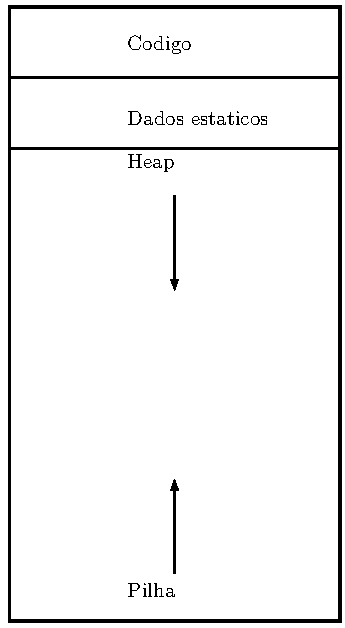
\includegraphics[scale=0.6]{memoria.pdf}
    \end{center}

\end{frame}

%%%%%%%%%%%%%%%%%%%%%%%%%%%%%%%%%%%%%%%%%%%%%%
\begin{frame}[fragile]{Organização da memória do computador}

    \small
    Em C99 podemos declarar vetores de tamanho variável em tempo de execução usando o valor de uma variável.

    No exemplo abaixo declaramos o vetor \cod{v} com tamanho igual ao valor da variável \cod{n}, que foi lida do teclado.
    \vspace{-0.3cm}

    \begin{minted}[fontsize=\scriptsize]{c}
        #include <stdio.h>
        int main() {
            long int n, i;

            scanf("%ld", &n);
            double v[n]; /* Vetor alocado com tamanho n não pré-estabelecido */

            for (i = 0; i < n; i++)
                v[i] = i;
            for (i = 0; i < n; i++) 
                printf("%.2lf\n", v[i]);
            return 0;
        }
     \end{minted}

\end{frame}

%%%%%%%%%%%%%%%%%%%%%%%%%%%%%%%%%%%%%%%%%%%%%%
\begin{frame}[fragile]{Organização da memória do computador}

    \small
    Porém, a criação de vetores desta forma faz a alocação de memória na \textbf{pilha}, que possui um limite máximo.

    Execute o programa a seguir digitando 1000000 e depois 2000000.
    \vspace{-0.3cm}
    \begin{minted}[fontsize=\scriptsize]{c}
        #include <stdio.h>
        int main() {
            long int n, i;

            scanf("%ld", &n);
            double v[n]; /* Vetor alocado com tamanho n não pré-estabelecido */

            for (i = 0; i < n; i++)
                v[i] = i;
            for (i = 0; i < n; i++) 
                printf("%.2lf\n", v[i]);
            return 0;
        }
     \end{minted}

\end{frame}

%%%%%%%%%%%%%%%%%%%%%%%%%%%%%%%%%%%%%%%%%%%%%%
\begin{frame}[fragile]{Organização da memória do computador}

    \begin{itemize}
        \item O programa anterior será encerrado ({\it segmentation fault}) se for usado um valor grande o suficiente para $n$.
        \item Isto se deve ao fato de que o SO limita o que pode ser alocado na pilha na execução de uma função.
        \item Este limite não existe para o Heap (com exceção do limite de memória do computador).
    \end{itemize}

\end{frame}

%%%%%%%%%%%%%%%%%%%%%%%%%%%%%%%%%%%%%%%%%%%%%%
\begin{frame}[fragile]{Organização da memória do computador}

    Utilizando alocação dinâmica não temos o problema de erro do programa anterior.
    \vspace{-0.3cm}

    \begin{minted}{c}
        #include <stdio.h>
        #include <stdlib.h>
        
        int main() {
            long int n = 2000000, i;
            double *v = malloc(n * sizeof(double));
            for (i = 0; i < n; i++)
                v[i] = i;
            for (i = 0; i < n; i++)
                printf("%.2lf\n", v[i]);
            free(v);
            return 0;
        }
    \end{minted}

\end{frame}

%%%%%%%%%%%%%%%%%%%%%%%%%%%%%%%%%%%%%%%%%%
%%%%%%%%%%%%%%%%%%%%%%%%%%%%%%%%%%%%%%%%%%
%%%%%%%%%%%%%%%%%%%%%%%%%%%%%%%%%%%%%%%%%%
%%%%%%%%%%%%%%%%%%%%%%%%%%%%%%%%%%%%%%%%%%
%%%%%%%%%%%%%%%%%%%%%%%%%%%%%%%%%%%%%%%%%%
%%%%%%%%%%%%%%%%%%%%%%%%%%%%%%%%%%%%%%%%%%
\section{Exemplos de ponteiros e alocação dinâmica}

%%%%%%%%%%%%%%%%%%%%%%%%%%%%%%%%%%%%%%%%%%%%%%
\begin{frame}[fragile]{Exemplo de ponteiros e alocação dinâmica}
    
    Vamos criar uma aplicação que usa vetores dinâmicos e implementa as seguintes operações:

    \begin{itemize}
        \item Inclusão de um elemento no final do vetor.
        \item Exclusão da primeira ocorrência de um elemento no vetor.
        \item Impressão do vetor.
    \end{itemize}

\end{frame}

%%%%%%%%%%%%%%%%%%%%%%%%%%%%%%%%%%%%%%%%%%%%%%
\begin{frame}[fragile]{Exemplo de ponteiros e alocação dinâmica}

    \begin{itemize}[<+->]
        \item O tamanho do vetor deve se ajustar automaticamente: se elementos são inseridos, devemos ``aumentar'' o tamanho do vetor para inclusão de novos elementos, e se elementos forem removidos devemos ``diminuir'' o tamanho vetor.

        \item Temos duas variáveis associadas ao vetor:
        \begin{itemize}
            \item \cod{tam}: denota quantos elementos estão armazenados no vetor. 
            \item \mintinline{c}{max_tam}: denota o tamanho alocado do vetor.
        \end{itemize}
  \end{itemize}

\end{frame}

%%%%%%%%%%%%%%%%%%%%%%%%%%%%%%%%%%%%%%%%%%%%%%
\begin{frame}[fragile]{Exemplo de ponteiros e alocação dinâmica}

    Temos as seguintes regras para ajuste do tamanho alocado do vetor:
    \begin{itemize}
        \item O vetor deve ter tamanho alocado de pelo menos 4.
        \item Se o vetor ficar cheio, então devemos alocar um novo vetor com o dobro do tamanho atual.
        \item Se o número de elementos armazenados no vetor for menor do que 1/4 do tamanho alocado do vetor, então devemos alocar um novo vetor com metade do tamanho atual.
    \end{itemize}

\end{frame}

%%%%%%%%%%%%%%%%%%%%%%%%%%%%%%%%%%%%%%%%%%%%%%
\begin{frame}[fragile]{Exemplo de ponteiros e alocação dinâmica}

    \small
    Implementaremos as seguintes funções:
    \vspace{-0.3cm}

    \begin{minted}{c}
        int *cria_vet(int *tam, int *max_tam);
    \end{minted}
    \vspace{-0.3cm}
    Aloca um vetor inicial de tamanho 4, inicializando \cod{tam} com valor 0, \mintinline{c}{max_tam} com valor 4, e devolvendo o endereço do vetor alocado.
    \vspace{-0.3cm}

    \pause
    \begin{minted}{c}
        void imprime_vet(int *v, int tam, int max_tam);
    \end{minted}
    \vspace{-0.3cm}
    Imprime o conteúdo e tamanhos associados ao vetor \cod{v}.
    \vspace{-0.3cm}

    \pause
    \begin{minted}{c}
        int *adiciona(int *v, int *tam, int *max_tam, int elem);
    \end{minted}
    \vspace{-0.3cm}
    Adiciona o elemento \cod{elem} no final do vetor \cod{v}.
    Caso não haja espaço, um novo vetor com o dobro do tamanho deve ser alocado.
    A função sempre retorna o endereço do vetor, sendo o novo alocado ou o atual.
    Além disso, os valores de \cod{tam} e \mintinline{c}{max_tam} devem ser atualizados.

\end{frame}

%%%%%%%%%%%%%%%%%%%%%%%%%%%%%%%%%%%%%%%%%%%%%%
\begin{frame}[fragile]{Exemplo de ponteiros e alocação dinâmica}

    \small
    Implementaremos as seguintes funções:
    \vspace{-0.3cm}

    \begin{minted}{c}
        int busca(int *v, int tam, int elem);
    \end{minted}
    \vspace{-0.3cm}
    Determina se o elemento \cod{elem} está presente ou não no vetor \cod{v}.
    Caso esteja presente, retorna a posição da primeira ocorrência de \cod{elem} em \cod{v}.
    Caso contrário, retorna -1.
    \vspace{-0.3cm}
    
    \pause
    \begin{minted}{c}
        int *remove(int *v, int *tam, int *max_tam, int elem);
    \end{minted}
    \vspace{-0.3cm}
    Remove a primeira ocorrência do elemento \cod{elem} do vetor \cod{v}, caso este esteja presente.
    O valor de \cod{tam} deve ser decrementado de 1.
    Caso o número de elementos armazenados seja menor do que $\frac{1}{4} \mbox{\mintinline{c}{max_tam}}$, então um novo vetor de tamanho $\frac{1}{2} \mbox{\mintinline{c}{max_tam}}$ deve ser alocado no lugar de \cod{v}.
    A função sempre retorna o endereço inicial do vetor, sendo um novo vetor alocado ou não. 

\end{frame}

%%%%%%%%%%%%%%%%%%%%%%%%%%%%%%%%%%%%%%%%%%%%%%
\begin{frame}[fragile]{Exemplo de ponteiros e alocação dinâmica}

    \begin{minted}[fontsize=\scriptsize]{c}
        /* Cria vetor com tamanho total 4. Devolve o endereço do vetor criado. */
        int *cria_vet(int *tam, int *max_tam) {
            int *v = malloc(4 * sizeof(int));
            *tam = 0;
            *max_tam = 4;
            return v;
        }

        /* Imprime o vetor. */
        void imprime_vet(int *v, int tam, int max_tam) {
            int i;
            printf("Vetor de tamanho %d (max. alocado %d):\n", tam, max_tam);
            printf("%d", v[0]);
            for (i = 1; i < tam; i++)
                printf(", %d", v[i]);
            printf("\n");
        }
    \end{minted}

\end{frame}

%%%%%%%%%%%%%%%%%%%%%%%%%%%%%%%%%%%%%%%%%%%%%%
\begin{frame}[fragile]{Exemplo de ponteiros e alocação dinâmica}

    \begin{minted}[fontsize=\scriptsize]{c}
        int *adiciona(int *v, int *tam, int *max_tam, int elem) {
            if (*tam < *max_tam) {
                /* Tem espaço para o novo elemento. */
                v[*tam] = e;
                (*tam)++;
                return v;
            } else {
                /* Precisamos alocar um espaço maior. */
                ...
            }
        }
    \end{minted}

\end{frame}

%%%%%%%%%%%%%%%%%%%%%%%%%%%%%%%%%%%%%%%%%%%%%%
\begin{frame}[fragile]{Exemplo de ponteiros e alocação dinâmica}

    \begin{minted}[fontsize=\scriptsize]{c}
        int *adiciona(int *v, int *tam, int *max_tam, int elem) {
            if (*tam < *max_tam) {
                /* Tem espaco para o novo elemento. */
                ...
            } else {
                /* Precisamos alocar um espaço maior. */
                int *vaux = malloc(2 * (*max_tam) * (sizeof(int)));
                int i;
                for (i = 0; i < *tam; i++) /* Salva dados de v em vaux. */
                    vaux[i] = v[i];
                vaux[*tam] = e; /* Adiciona elemento no fim. */
                (*tam)++;
                *max_tam = 2 * (*max_tam); /* Atualiza dados de tamanho. */
                
                free(v); /* Libera memória não mais necessária. */
                return vaux;
            }
        }
    \end{minted}

\end{frame}

%%%%%%%%%%%%%%%%%%%%%%%%%%%%%%%%%%%%%%%%%%%%%%
\begin{frame}[fragile]{Exemplo de ponteiros e alocação dinâmica}

    \begin{minted}[fontsize=\scriptsize]{c}
        /* Retorna posição da primeira ocorrência de elem ou -1 caso elem não seja encontrado. */
        int busca(int *v, int tam, int elem) {
            int i;
            for (i = 0; i < tam; i++)
                if (v[i] == elem)
                    return i;
            return -1;
        }
    \end{minted}

\end{frame}

%%%%%%%%%%%%%%%%%%%%%%%%%%%%%%%%%%%%%%%%%%%%%%
\begin{frame}[fragile]{Exemplo de ponteiros e alocação dinâmica}

    \begin{minted}[fontsize=\scriptsize]{c}
        int *remove(int *v, int *tam, int *max_tam, int elem) {
            int i;
            i = busca(v, *tam, elem);
            if (i != -1) {
                /* O elemento está em v. */
                /* Copia dados a partir da posição i+1 uma posição para trás. */
                for (; i < (*tam)-1; i++)
                    v[i] = v[i+1];
                (*tam)--;

                /* Se tamanho do vetor for > 4 e ele estiver menos de 1/4 ocupado devemos diminuir tamanho do vetor pela metade. */
                if (*tam < (0.25 * (*max_tam)) && *max_tam > 4) {
                    ...
                    /* Exercício. */
                } 
            }
            return v;
        }
    \end{minted}

\end{frame}

%%%%%%%%%%%%%%%%%%%%%%%%%%%%%%%%%%%%%%%%%%%%%%
\begin{frame}[fragile]{Exemplo de ponteiros e alocação dinâmica}

    Com essas funções podemos executar o seguinte exemplo:
    \vspace{-0.3cm}
    \begin{minted}[fontsize=\scriptsize]{c}
        int main() {
            int *vet, tam, max_tam, i;
            vet = cria_vet(&tam, &max_tam);
            
            for (i = 0; i < 20; i++)
                vet = adiciona(vet, &tam, &max_tam, i);
            imprime_vet(vet, tam, max_tam);

            vet = remove(vet, &tam, &max_tam, 14);
            imprime_vet(vet, tam, max_tam);
            for (i = 5; i < 15; i++)
                vet = remove(vet, &tam, &max_tam, i);
            imprime_vet(vet, tam, max_tam);

            for (i = 0; i < 20; i++)
                vet = adiciona(vet, &tam, &max_tam, i);
            imprime_vet(vet, tam, max_tam);
            
            free(vet);
            return 0;
        }
    \end{minted}

\end{frame}


%%%%%%%%%%%%%%%%%%%%%%%%%%%%%%%%%%%%%%%%%%%%%%
%%%%%%%%%%%%%%%%%%%%%%%%%%%%%%%%%%%%%%%%%%%%%%
%%%%%%%%%%%%%%%%%%%%%%%%%%%%%%%%%%%%%%%%%%%%%%
%%%%%%%%%%%%%%%%%%%%%%%%%%%%%%%%%%%%%%%%%%%%%%
%%%%%%%%%%%%%%%%%%%%%%%%%%%%%%%%%%%%%%%%%%%%%%
%%%%%%%%%%%%%%%%%%%%%%%%%%%%%%%%%%%%%%%%%%%%%%
\section{Informações extras: ponteiros para ponteiros e alocação dinâmica de matrizes}

%%%%%%%%%%%%%%%%%%%%%%%%%%%%%%%%%%%%%%%%%%%%%%
\begin{frame}[fragile]{Informações extras: alocação dinâmica de matrizes}

    \begin{itemize}
        \item Em aplicações científicas e de engenharias, é muito comum a realização de diversas operações sobre matrizes.
        \item Em situações reais o ideal é alocar memória suficiente para conter os dados a serem tratados. Não usar nem mais e nem menos!
        \item Como alocar vetores multidimensionais dinamicamente?
    \end{itemize}

\end{frame}

%%%%%%%%%%%%%%%%%%%%%%%%%%%%%%%%%%%%%%%%%%%%%%
\begin{frame}[fragile]{Informações extras: ponteiros para ponteiros}

    \begin{itemize}
        \item Uma variável ponteiro está alocada na memória do computador como qualquer outra variável.
        \item Portanto, podemos criar um ponteiro que contém o endereço de memória de um outro ponteiro.
        \item Para criar um ponteiro para ponteiro: \cod{tipo **nomePonteiro;}
        
        \begin{minted}{c}
            int main() {
                int a = 5, *b, **c;
                b = &a;
                c = &b;
                printf("%d\n", a);
                printf("%d\n", *b);
                printf("%d\n", *(*c));
                return 0;
            }
        \end{minted}
    \end{itemize}

\end{frame}

%%%%%%%%%%%%%%%%%%%%%%%%%%%%%%%%%%%%%%%%%%%%%%
\begin{frame}[fragile]{Informações extras: ponteiros para ponteiros}

    O programa imprime 5 três vezes, mostrando as três formas de acesso à variável \cod{a}: \cod{a, *b, **c}.

    \begin{center}
        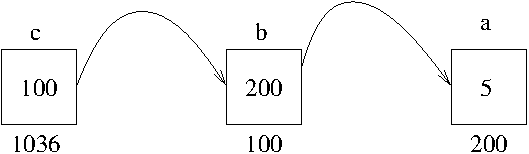
\includegraphics[scale=0.8]{pont2}
    \end{center}

\end{frame}

%%%%%%%%%%%%%%%%%%%%%%%%%%%%%%%%%%%%%%%%%%%%%%
\begin{frame}[fragile]{Informações extras: ponteiros para ponteiros}

    Pela nossa discussão anterior sobre ponteiros, sabemos que um ponteiro pode ser usado para referenciar um vetor alocado dinamicamente.
    
    \begin{minted}{c}
        int *p;
        p = calloc(5, sizeof(int));
    \end{minted}
    
    \begin{center}
        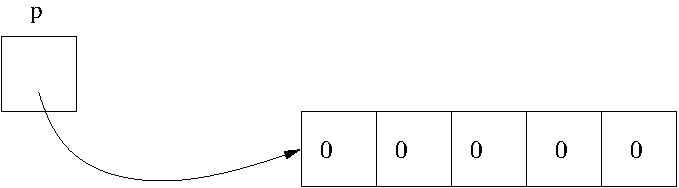
\includegraphics[scale=0.8]{pont3}
    \end{center}

\end{frame}

%%%%%%%%%%%%%%%%%%%%%%%%%%%%%%%%%%%%%%%%%%%%%%
\begin{frame}[fragile]{Informações extras: ponteiros para ponteiros}

    A mesma coisa acontece com um ponteiro para ponteiro, só que neste caso o vetor alocado é de ponteiros.

    \begin{minted}{c}
        int **p;
        p = calloc(5, sizeof(int *));
    \end{minted}

    \begin{center}
        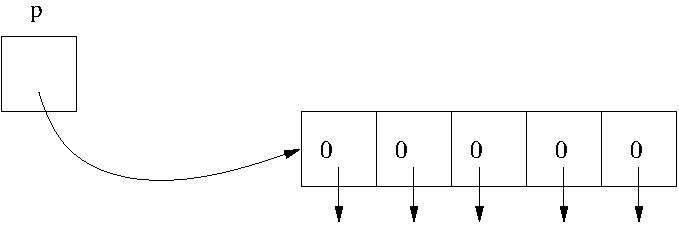
\includegraphics[scale=0.8]{pont4}
    \end{center}

    Note que cada posição do vetor acima é do tipo \cod{int *}, ou seja, um ponteiro para inteiro!

\end{frame}

%%%%%%%%%%%%%%%%%%%%%%%%%%%%%%%%%%%%%%%%%%%%%%
\begin{frame}[fragile]{Informações extras: ponteiros para ponteiros}

    Como cada posição do vetor é um ponteiro para inteiro, podemos associar cada posição dinamicamente com um vetor de inteiros.
    \begin{minipage}{0.5\textwidth}
        \begin{minted}[fontsize=\scriptsize]{c}
            int **p;
            int i;
            p = calloc(5, sizeof(int *));
            for (i = 0; i < 5; i++)
                p[i] = calloc(3, sizeof(int));
        \end{minted}
    \end{minipage}
    \begin{minipage}{0.45\textwidth}
        \begin{center}
            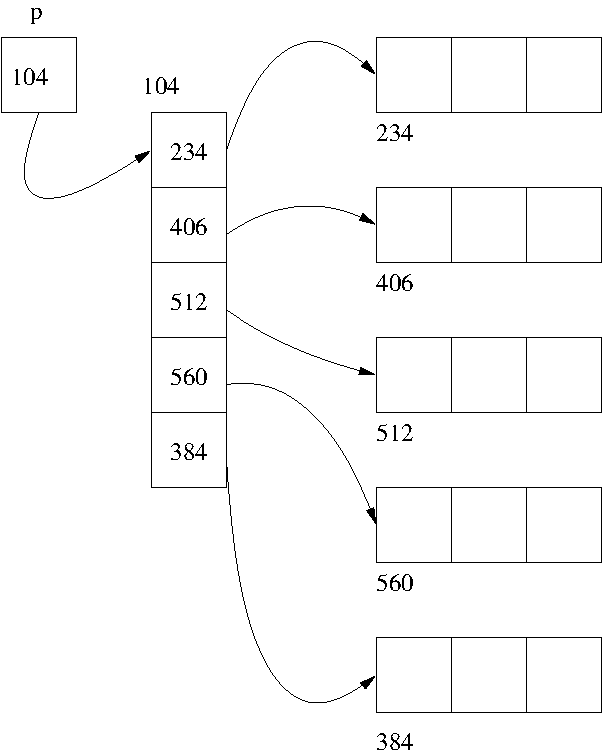
\includegraphics[width=\textwidth]{pont5}
        \end{center}
    \end{minipage}

\end{frame}

%%%%%%%%%%%%%%%%%%%%%%%%%%%%%%%%%%%%%%%%%%%%%%
\begin{frame}[fragile]{Informações extras: alocação dinâmica de matrizes}

    Esta é uma forma de se criar matrizes dinamicamente:
    \begin{itemize}
        \item Crie um ponteiro para ponteiro.
        \item Associe um vetor de ponteiros dinamicamente com este ponteiro de ponteiro. O tamanho deste vetor é o número de linhas da matriz.
        \item Cada posição do vetor será associada com um outro vetor do tipo a ser armazenado. Cada um destes vetores é uma linha da matriz (portanto possui tamanho igual ao número de colunas).
    \end{itemize}
    
    \alert{OBS: No final você deve desalocar toda a memória alocada!!}

\end{frame}

%%%%%%%%%%%%%%%%%%%%%%%%%%%%%%%%%%%%%%%%%%%%%%
\begin{frame}[fragile]{Informações extras: alocação dinâmica de matrizes}

    \begin{minted}[fontsize=\tiny]{c}
        int main() {
            int **p, i, j;
            
            p = calloc(5, sizeof(int *));
            for (i = 0; i < 5; i++)
                p[i] = calloc(3, sizeof(int));
            /* Alocou matriz 5x3 acima */

            printf("Digite os valores da matriz\n");
            for (i = 0; i < 5; i++)
                for (j = 0; j < 3; j++)
                    scanf("%d", &p[i][j]);

            printf("Matriz lida\n");
            for (i = 0; i < 5; i++) {
                for (j = 0; j < 3; j++)
                    printf("%d, ", p[i][j]);
                printf("\n");
            }

            /* Desalocando a memória usada: */
            for (i = 0; i < 5; i++)
                free(p[i]);
            free(p);
            return 0;
        }
    \end{minted}

\end{frame}


%%%%%%%%%%%%%%%%%%%%%%%%%%%%%%%%%%%%%%%%%%%%%%
%%%%%%%%%%%%%%%%%%%%%%%%%%%%%%%%%%%%%%%%%%%%%%
%%%%%%%%%%%%%%%%%%%%%%%%%%%%%%%%%%%%%%%%%%%%%%
%%%%%%%%%%%%%%%%%%%%%%%%%%%%%%%%%%%%%%%%%%%%%%
%%%%%%%%%%%%%%%%%%%%%%%%%%%%%%%%%%%%%%%%%%%%%%
%%%%%%%%%%%%%%%%%%%%%%%%%%%%%%%%%%%%%%%%%%%%%%
\section{Exercícios}

%%%%%%%%%%%%%%%%%%%%%%%%%%%%%%%%%%%%%%%%%%%%%%
\begin{frame}[fragile]{\exercicio}

    Qual o resultado da execução do programa abaixo? Ocorre algum erro?
    \vspace{-0.3cm}
    \begin{minted}[fontsize=\tiny]{c}
        #include <stdio.h>
        #include <stdlib.h>

        int *misterio(int n) {
            int i, *vet;

            vet = malloc(n * sizeof(int));
            
            vet[0] = 1;
            for (i = 1; i < n; i++) 
                vet[i] = i * vet[i-1];
            
            return vet;
        }
        
        int main() {
            int i, n, *v;
            scanf("%d", &n);
            v = misterio(n);
            for (i = 0; i < n; i++)
                printf("%d\n", v[i]);
            free(v);
            return 0;
        }
    \end{minted}

\end{frame}

%%%%%%%%%%%%%%%%%%%%%%%%%%%%%%%%%%%%%%%%%%%%%%
\begin{frame}[fragile]{\exercicio}

    Faça um programa que lê a dimensão $n$ de um vetor, em seguida aloca dinamicamente dois vetores do tipo {\it double} de dimensão $n$, faz a leitura de cada vetor e, finalmente, imprime o resultado da soma dos dois vetores.

\end{frame}

%%%%%%%%%%%%%%%%%%%%%%%%%%%%%%%%%%%%%%%%%%%%%%
\begin{frame}[fragile]{\exercicio}

    Faça uma função que recebe como parâmetro dois vetores de inteiros representando conjuntos de números inteiros e devolve um outro vetor com o resultado da união dos dois conjuntos.
    
    O vetor resultante deve ser alocado dinamicamente.

    O protótipo da função é
    \begin{minted}{c}
        int *uniao(int *v1, int n1, int *v2, int n2);
    \end{minted}

    onde {\bf n1} e {\bf n2} indicam o número de elementos em {\bf v1} e {\bf v2}, respectivamente.

\end{frame}

%%%%%%%%%%%%%%%%%%%%%%%%%%%%%%%%%%%%%%%%%%%%%%
\begin{frame}[fragile]{\exercicio}

    Vimos uma aplicação que aumenta e diminui o tamanho do vetor conforme necessário durante a execução.

    Implemente a função de remoção de um elemento do vetor.
    
\end{frame}

%%%%%%%%%%%%%%%%%%%%%%%%%%%%%%%%%%%%%%%%%%
%%%%%%%%%%%%%%%%%%%%%%%%%%%%%%%%%%%%%%%%%%
%%%%%%%%%%%%%%%%%%%%%%%%%%%%%%%%%%%%%%%%%%
%%%%%%%%%%%%%%%%%%%%%%%%%%%%%%%%%%%%%%%%%%
%%%%%%%%%%%%%%%%%%%%%%%%%%%%%%%%%%%%%%%%%%
%%%%%%%%%%%%%%%%%%%%%%%%%%%%%%%%%%%%%%%%%%
\section{Informações extras: alocação dinâmica de matrizes}

%%%%%%%%%%%%%%%%%%%%%%%%%%%%%%%%%%%%%%%%%%%%%%
\begin{frame}[fragile]{Informações extras: alocação dinâmica de matrizes}

    Vimos que alocar ponteiros para ponteiros é uma forma de se fazer alocação dinâmica de matrizes.

    Mas a forma mais eficiente de criar matrizes é:
    \begin{itemize}
        \item Para uma matriz de dimensões $n \times m$, crie dinamicamente um vetor \textit{unidimensional} deste tamanho.
        \item Use linearização de índices para trabalhar com o vetor como se fosse uma matriz.
        \item Desta forma, tem-se um melhor aproveitamento da cache pois a matriz inteira está sequencialmente em memória.
    \end{itemize}

    No final você deve desalocar toda a memória alocada!!

\end{frame}

%%%%%%%%%%%%%%%%%%%%%%%%%%%%%%%%%%%%%%%%%%%%%%%
\begin{frame}[fragile]{Linearização de índices}

    \begin{itemize}
        \item Podemos sempre usar vetores simples para representar matrizes (na prática o compilador faz isto por você).
        \item Ao declarar uma matriz como \cod{int mat[3][4]}, sabemos que serão alocadas 12 posições de memória associadas com a variável \cod{mat}.
        \item Poderíamos simplesmente criar \cod{int mat[12]} então.
        \item Apenas perderíamos a simplicidade de uso dos índices em forma de matriz.
        \begin{itemize}
            \item Você não poderá escrever \cod{mat[1][3]}, por exemplo.
        \end{itemize}
    \end{itemize}

\end{frame}

%%%%%%%%%%%%%%%%%%%%%%%%%%%%%%%%%%%%%%%%%%%%%%%
\begin{frame}[fragile]{Linearização de índices}

    \begin{itemize}
        \item A {\it linearização de índices} é justamente a representação de matrizes usando-se um vetor simples.
        \item Mas devemos ter um padrão para acessar as posições deste vetor como se sua organização fosse na forma de matriz.
    \end{itemize}

\end{frame}

%%%%%%%%%%%%%%%%%%%%%%%%%%%%%%%%%%%%%%%%%%%%%%%
\begin{frame}[fragile]{Linearização de índices}

    \begin{itemize}
        \item Considere o exemplo: \cod{int mat[12]; /* ao invés de int mat[3][4] */}
        \item Fazemos a divisão por linhas como segue:
        \begin{itemize}
            \item Primeira linha: \cod{mat[0]} até \cod{mat[3]} 
            \item Segunda linha: \cod{mat[4]} até \cod{mat[7]} 
            \item Terceira linha: \cod{mat[8]} até \cod{mat[11]} 
        \end{itemize}
        \item Para acessar uma posição ``\cod{[i][j]}'', usamos:
        \begin{itemize}
            \item  \cod{mat[i*4 + j];} onde $0 \le i \le 2$ e $0 \le j \le 3$. 
        \end{itemize}
    \end{itemize}

\end{frame}

%%%%%%%%%%%%%%%%%%%%%%%%%%%%%%%%%%%%%%%%%%%%%%%
\begin{frame}[fragile]{Linearização de índices}

    \begin{itemize}
        \item De forma geral, seja matriz \cod{mat[n*m]}, representando \cod{mat[n][m]}.
        \item Para acessar a posição correspondente à \cod{[i][j]} usamos:
        \begin{itemize}
            \item  \cod{mat[i*m + j];} onde $0 \le i \le n-1$  e $0 \le j \le m-1$.
        \end{itemize}
        \item Note que $i$ pula de blocos de tamanho $m$, e $j$ indexa a posição dentro de um bloco.
    \end{itemize}

\end{frame}

%%%%%%%%%%%%%%%%%%%%%%%%%%%%%%%%%%%%%%%%%%%%%%%
\begin{frame}[fragile]{Linearização de índices}

    \begin{minted}{c}
        int main() {
            int mat[40]; /* representando mat[5][8] */
            int i, j;
            
            for (i = 0; i < 5; i++)
                for (j = 0; j < 8; j++)
                    mat[i*8 + j] = i*j;

            for (i = 0; i < 5; i++) {
                for (j = 0; j < 8; j++)
                    printf("%d, ", mat[i*8 + j]);
                printf("\n");
            }

            return 0;
        }
    \end{minted}

\end{frame}


\end{document}
